\documentclass[11pt,a4paper,makeidx]{book}

\usepackage[french]{babel}
\usepackage[utf8x]{inputenc}
\usepackage{subfig}
\usepackage{amsmath,amsthm,amssymb,pifont,makeidx,geometry}
\usepackage{makeidx}
\usepackage{color}
\usepackage[pagebackref=true,breaklinks=true,colorlinks,bookmarks=false]{hyperref}
\usepackage{graphicx}
\usepackage{wasysym,pifont}

\newcommand{\checkItem}{\textbf{\Pisymbol{wasy}{8}}\hspace{3mm}}
\newcommand{\command}[1]{\framebox[\textwidth][l]{\tt \$ #1}}
\newcommand{\fileName}[1]{{\tt #1}}
\newcommand{\commandName}[1]{\textcolor{red}{\tt #1}}
\newcommand{\optionName}[1]{\textcolor{green}{\tt #1}}
\newcommand{\outputName}[1]{\textcolor{blue}{\tt #1}}

\newcounter{thenote}
\newenvironment{note}{\stepcounter{thenote} \noindent \textcolor{red}{\textbf{Note \arabic{thenote}}~:}}{\par}
\newcommand{\warning}[1]{\textcolor{red}{\textbf{Attention~: #1}}}

\bibliographystyle{plain}

\graphicspath{{../images/}}
%\DeclareGraphicsRule{.jpg}{eps}{.ps.bb}{`convert #1 ps:-}
%\DeclareGraphicsRule{.gif}{eps}{.ps.bb}{`convert #1 ps:-}
%\DeclareGraphicsRule{.png}{eps}{.ps.bb}{`convert #1 ps:-}

\geometry{width=17cm,height=21.7cm}
\makeindex 

\title{{\textbf{\textcolor{blue}{Tutoriel\\
        {\Large Problème direct avec OpenMEEG.\\
                Utilisation par lignes de commande.}}}}}
\author{Maureen Clerc\\Alexandre Gramfort \\
        Perrine Landreau\\Théo Papadopoulo}

\date{08 Juin 2008\\
      Version 0.3}

\pdfpageattr {/Group << /S /Transparency /I true /CS /DeviceRGB>>}
\begin{document}

    \maketitle
    \tableofcontents

    \chapter{Contexte}
    \centerline{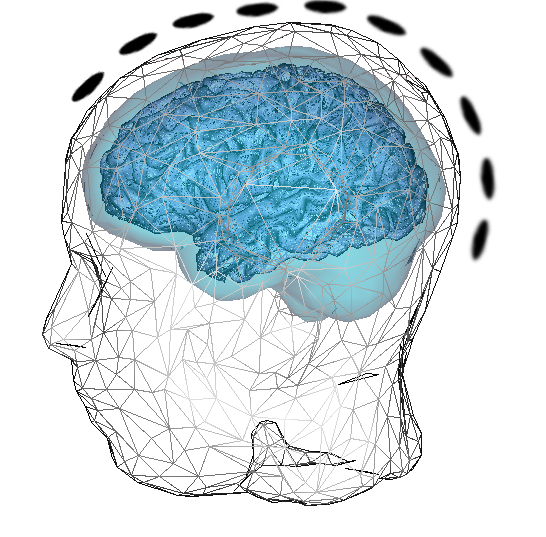
\includegraphics[height=9cm]{surf3.png}}

\noindent
Le problème direct consiste à estimer la valeur des potentiels et champs magnétiques qui seraient enregistrés \textbf{aux
capteurs} MEG/EEG étant donné une source d'activité.

\centerline{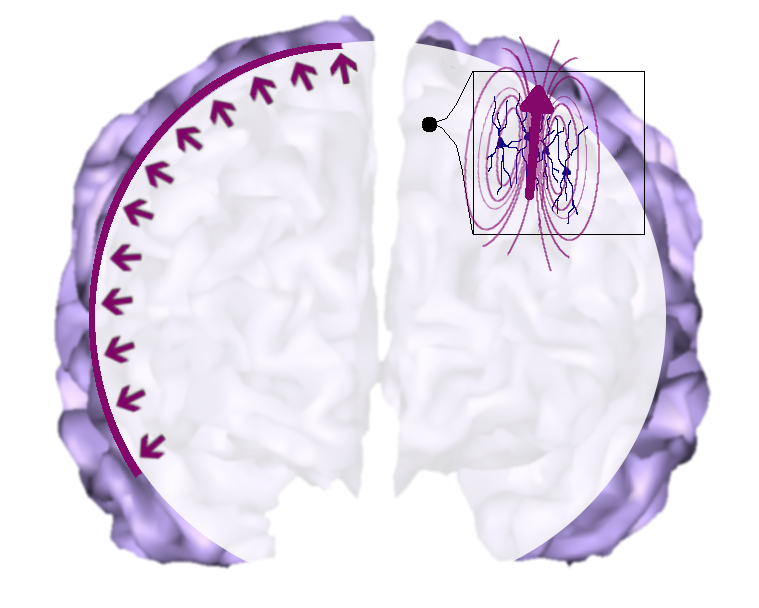
\includegraphics[height=10cm]{dipole.png}}

\noindent
\underline{Étape 1}~: on calcule le potentiel \textbf{sur toutes les surfaces } du modèle de tête (scalp, crâne extérieur et crâne intérieur pour un modèle à trois couches). Soit $\mathbf{X}$ un vecteur rassemblant  les valeurs du potentiel et des courants normaux sur les surfaces discrétisées. La méthode des éléments
frontières symétrique ramène à la résolution d'un système linéaire
suivant~:
\[
    \mathbf{HeadMat} . \mathbf{X} = \mathbf{SourceMat}
\]
Voir points \ref{sect: command assemble HeadMat}, \ref{sect: command assemble SourceMat} et \ref{sect: command invert HeadMat}.

\medskip

\noindent
\underline{Étape 2}~: les capteurs sont reliés au modèle de tête par plusieurs transformations linéaires représentées par des matrices. Ces matrices diffèrent entre la MEG et l'EEG. \\
\\
Pour l'EEG, le potentiel est interpolé aux positions des capteurs à partir des maillages de surfaces discrétisées, par une application linéaire~:\\
\[
    \left[ \mbox{valeur aux capteurs} \right] =
    \left[ \mbox{matrice de passage} \right] \times \left[ \mbox{valeurs sur le scalp} \right] \mbox{dans le cas de l'EEG.}
\]
Pour la MEG, l'équation de Biot et Savart montre qu'il y a deux contributions au champ magnétique: l'une provenant directement des sources d'activité électrique cérébrale, et l'autre provenant du courant ohmique, et calculable à partir du potentiel sur les surfaces du modèle.
Par conséquent, deux transformations linéaires doivent être calculées, l'une reliant les positions de sources aux capteurs MEG, et l'autre reliant les surfaces du modèle aux capteurs MEG.

Voir point \ref{sect: command assemble sensors}.

\medskip

\noindent
\underline{Étape 3}~: la matrice reliant les sources (à \textbf{position et orientation} fixée)  aux capteurs peut désormais être calculée. Cette matrice
est appelée matrice de gain et notée $\mathbf{G}$~ (point \ref{sect: command gain}). 
Appliquée à une matrice reflétant l'\textbf{activation} des sources, elle donne la solution du problème direct (point
\ref{sect: command direct}).


    \chapter{Données}
    \noindent

Dans cette partie nous décrivons les grands types de données sur lesquelles repose le calcul du problème direct par OpenMEEG.
Pour des détails sur les structures de données, on se reportera à l'Annexe~\ref{chap:formats}.

\noindent
\underline{Maillages}~:\\
il faut définir des maillages pour les interfaces des différents domaines de conductivité. Il s'agit, généralement de trois maillages~:
\begin{itemize}
    \item un maillage grossier de la surface extérieure du cortex,
    \item un maillage de la surface extérieure du crâne,
    \item un maillage pour la surface extérieure scalp.
\end{itemize}

\noindent
La taille recommandée pour ces maillages est d'environ 600 à 800 points par surface.

\medskip

\centerline{
    \hbox{\parbox[t]{5.5cm}{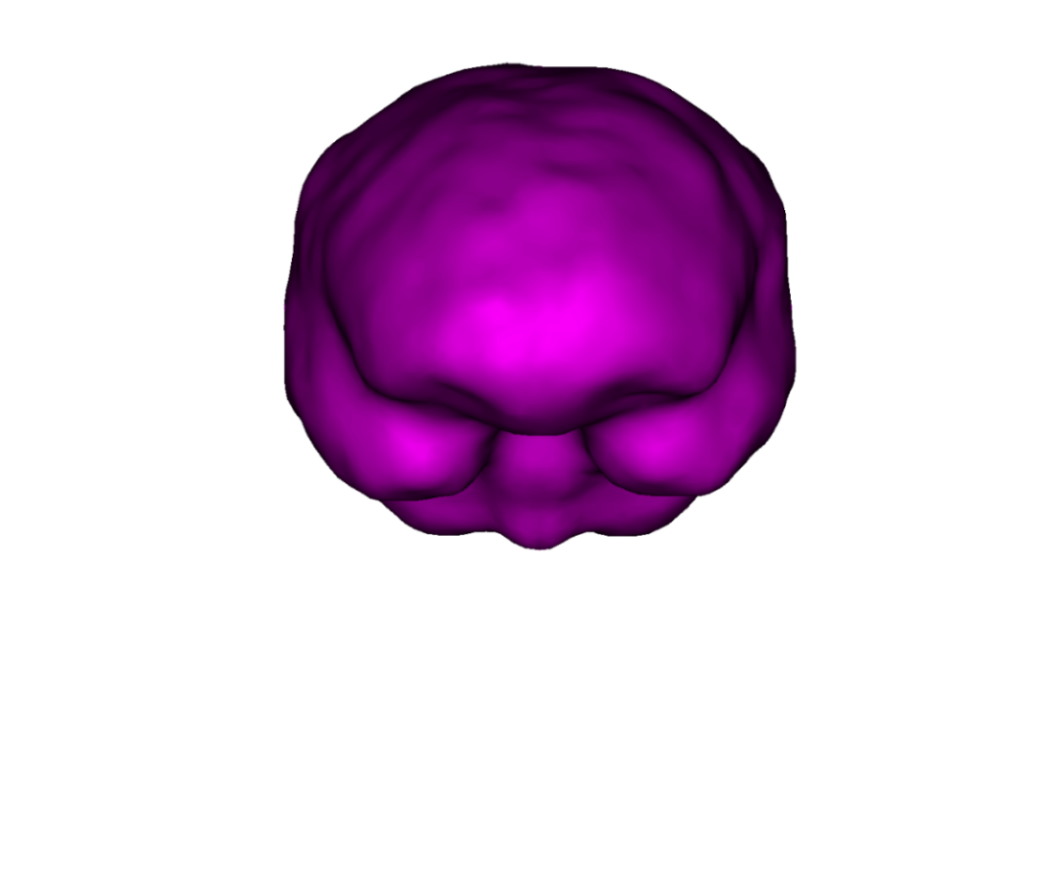
\includegraphics[width=5cm]{tete_couches_brain.png}\\
                            \parbox{5cm}{Surface extérieure au cortex}}
          \parbox[t]{5.5cm}{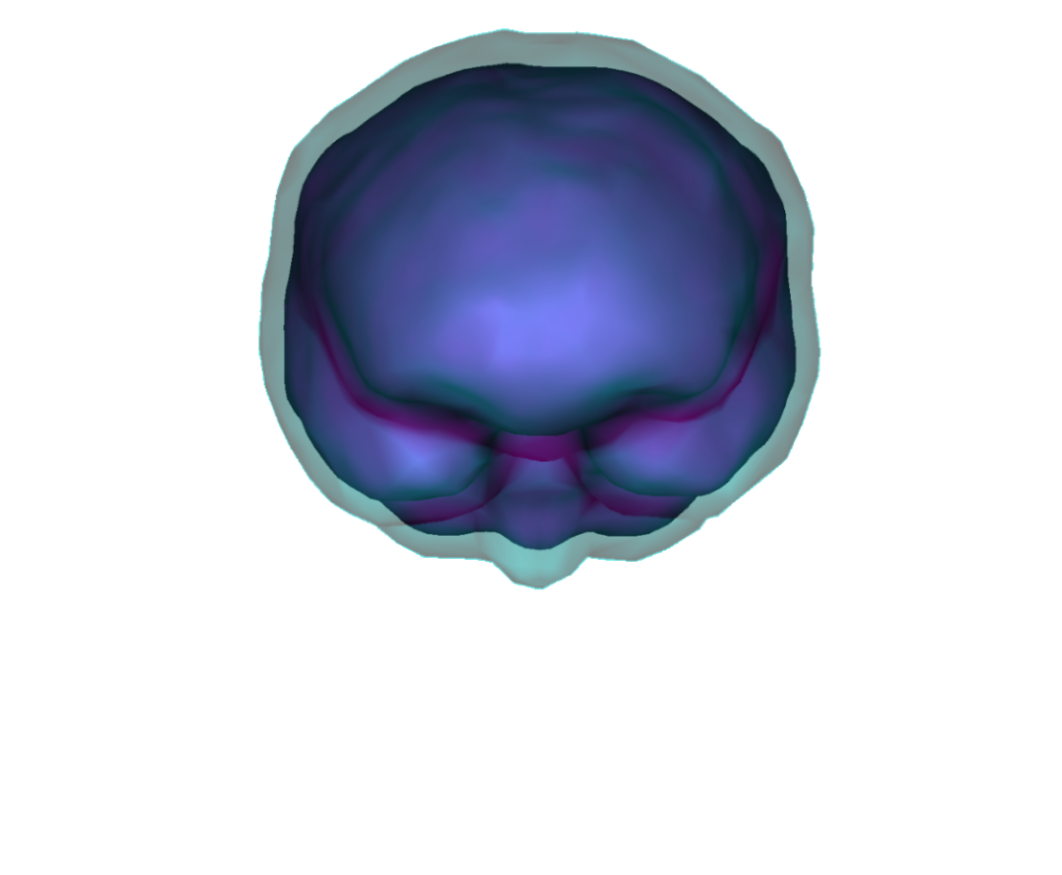
\includegraphics[width=5cm]{tete_couches_brainskull.png}\\\parbox{5cm}{Surface extérieure au crâne en bleu et surface extérieure au cortex en fushia}}
          \parbox[t]{5.5cm}{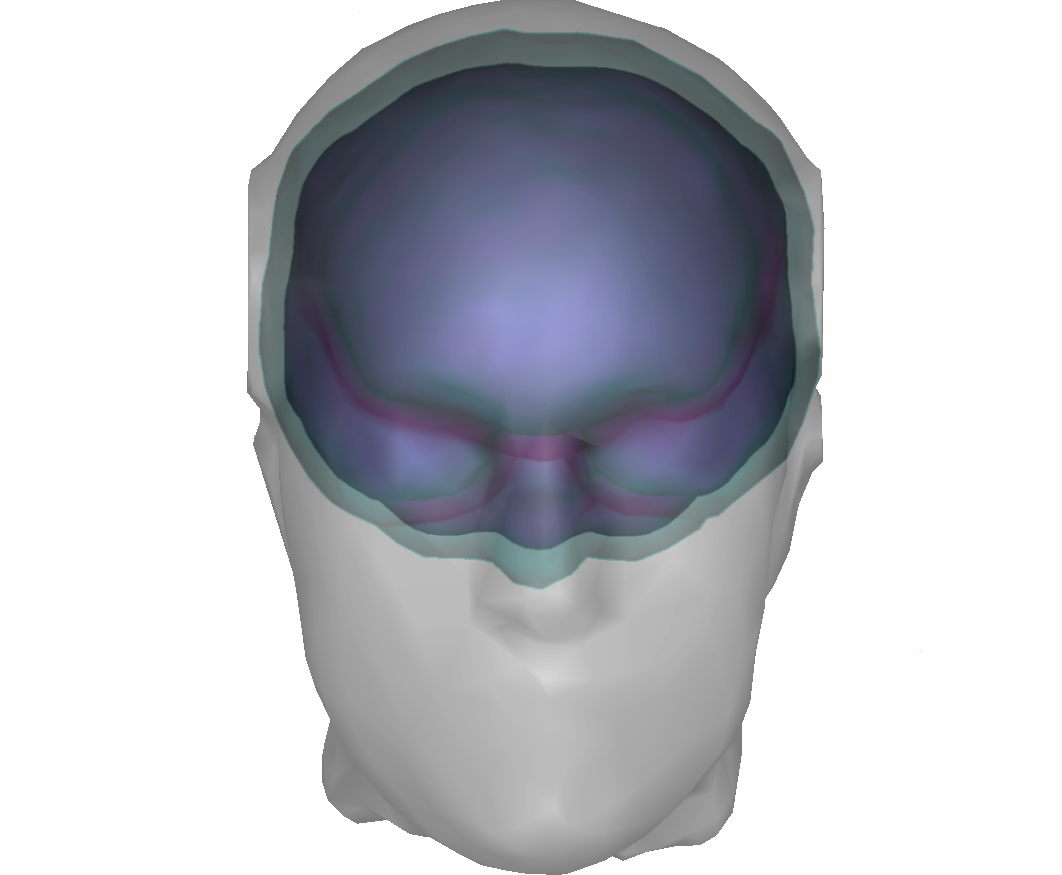
\includegraphics[width=5cm]{tete_couches_brainskullhead.png}\\
                            \parbox{5cm}{Exemple avec trois surfaces~:
                                  \begin{itemize}
                                       \item extérieure au scalp en gris
                                       \item extérieure au crâne en bleu
                                       \item extérieur au cortex en fushia
                                  \end{itemize}}
                            }
    }
}

\bigskip

\noindent
\underline{Sources}~:\\
Les sources peuvent être de deux types: isolées ou distribuées.
\noindent
Dans le cas de sources distribuées, il faut un maillage représentant le support des sources. Il s'agit généralement d'un maillage détaillé du cerveau, dont la taille peut varier de 10 000 et 30 000 points.
Les sources représentées par un maillage ont une amplitude  {\em continue} et linéaire sur chaque triangle de la surface maillée. Cette amplitude est discrétisée par des éléments finis P1 (polynomiaux de degré un).
L'orientation des sources est constante par morceaux, d'orientation normale à chaque triangle.
\begin{center}
    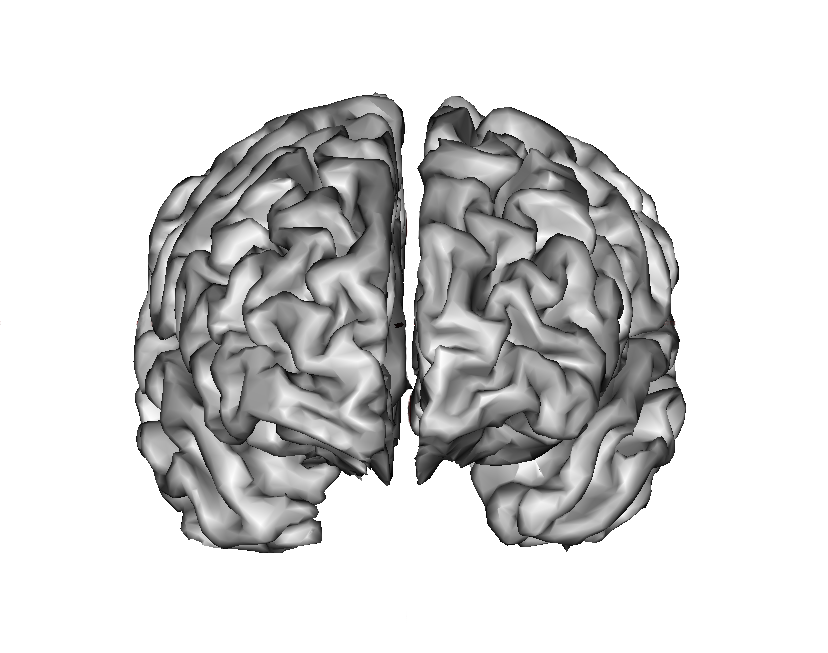
\includegraphics[height=9cm]{cortex.png}\\
    Maillage de sources
\end{center}
\noindent
Des sources isolées sont constituées d'une superposition de dipôles de courants ponctuels, chacun défini par sa position et son moment.

\noindent
\underline{Capteurs}~:
	Dans le cas de l'EEG, un fichier de description de la position des électrodes (ou patches) en coordonnées cartésiennes.
Dans le cas de la MEG, les capteurs sont plus complexes à décrire, cf l'Annexe~\ref{sec:sensors}.


    \chapter{Lignes de commande}
    \noindent
Sont en \commandName{rouge} les binaires appelés, en \optionName{vert} les options de ces binaires, en \textbf{noir}
les fichiers existants et en \outputName{bleu} les sorties/résultats. 

\section{Assemblage de la matrice $\mathbf{HeadMat}$~:}
\label{sect: command assemble HeadMat}

\noindent
Entrées~: 
\begin{itemize}
    \item \fileName{subject.geom}~: fichier de description de la géométrie (voir Annexe~\ref{sect: annexe 1})
    \item \fileName{subject.cond}~: fichier de description des conductivités (voir Annexe~\ref{sect: annexe 2})
\end{itemize}

\noindent
Sortie~:
\begin{itemize}
    \item \outputName{HeadMat.bin}~: fichier binaire où est sauvée la matrice $\mathbf{HeadMat}$
\end{itemize}

\medskip

\noindent
\command{\commandName{om\_assemble} \optionName{-HeadMat} subject.geom subject.cond \outputName{HeadMat.bin}}
\medskip
Remarque: \optionName{-HeadMat} peut être remplacé par la version abrégée \optionName{-HM} ou \optionName{-hm}.

\section{Assemblage de la matrice $\mathbf{Source}$~:}
\label{sect: command assemble SourceMat}

\noindent
Entrées~: 
\begin{itemize}
    \item \fileName{subject.geom}~: fichier de description de la géométrie (voir Annexe~\ref{sect: annexe 1})
    \item \fileName{subject.cond}~: fichier de description des conductivités (voir Annexe~\ref{sect: annexe 2})
    \item la/les source(s)~:
        \begin{description}
            \item [[cas dipolaire]] \fileName{dipolePosition.dip}~: fichier de localisation du/des dipole(s) (coordonnées et orientation)
                                    (voir Annexe~\ref{sect: annexe 3}) 
            \item [[cas des sources distribuées]]  \fileName{sourcemesh}~: maillage de sources (format *.tri de BrainVisa, ou *.mesh de BrainVisa, ou *.vtk de VTK) 
        \end{description}
\end{itemize}

\noindent
Sortie~:
\begin{itemize}
    \item \outputName{SourceMat.bin}~: fichier binaire matrice $\mathbf{SourceMat}$
\end{itemize}

\medskip

\noindent
Cas dipolaire~:\\
\noindent
\command{\commandName{om\_assemble} \optionName{-DipSourceMat} subject.geom subject.cond dipolePosition.dip \outputName{SourceMat.bin}}
\medskip
Remarque: \optionName{-DipSourceMat} peut être remplacé par la version abrégée \optionName{-DSM} ou \optionName{-dsm}.

\medskip

\noindent
Cas des sources distribuées~:\\
\noindent
\command{\commandName{om\_assemble} \optionName{-SurfSourceMat} subject.geom subject.cond sourcemesh \outputName{SourceMat.bin}}
\medskip
Remarque: \optionName{-SurfSourceMat} peut être remplacé par la version abrégée \optionName{-SSM} ou \optionName{-ssm}.

\section{Inversion de la matrice $\mathbf{HeadMat}$~:}
\label{sect: command invert HeadMat}

\noindent
Entrées~:
\begin{itemize}
    \item \fileName{HeadMat.bin}~: matrice $\mathbf{HeadMat}$
\end{itemize}

\noindent
Sortie~:
\begin{itemize}
    \item \outputName{HeadMatInv.bin}~: fichier binaire matrice $\mathbf{HeadMat}^{-1}$
\end{itemize}

\medskip

\noindent
\command{\commandName{om\_minverser} HeadMat.bin \outputName{HeadMatInv.bin}}

\section{Calcul de l'application linéaire qui à X associe le potentiel aux capteurs~:}
\label{sect: command assemble sensors}

\checkItem \underline{Cas de l'EEG}~:\\
"La méthode BEM symétrique fournit le potentiel électrique aux sommets des maillages de toutes les interfaces. Pour simuler le
potentiel à une électrode donnée, on projette sa position sur la dernière interface (censée modéliser le scalp) et on interpole
ensuite la valeur en ce point grâce aux fonctions P1.  [...] on considère [...] un modèle de tête ainsi que des positions de
capteurs EEG et MEG fixes par rapport à ce modèle. Le passage des valeurs du potentiel électrique de l'interface la plus externe
aux électrodes est donc une opération linéaire (par rapport aux valeurs du potentiel sur la dernière couche)."
\emph{\underline{\textcolor{blue}{Extrait de la thèse de Geoffray Adde "Méthodes de traitement d'image appliquées au}}}\\
\emph{\underline{\textcolor{blue}{problème inverse en magnéto-électro-encéphalographie"}}  p.62-63.}

\medskip

\noindent
On a alors~: $\mathbf{V_{electrode}} = \mathbf{Head2EEG} . \mathbf{X}$\\
où~:\\ 
\begin{itemize}
    \item $\mathbf{V_{electrode}}$ est le vecteur-colonne des valeurs du potentiel électrique aux électrodes (ce que l'on cherche),
    \item $\mathbf{X}$ est le vecteur-colonne contenant les valeurs du potentiel électrique et des courants normaux sur toutes les surfaces du modèle,
    \item $\mathbf{Head2EEG}$ est la matrice de passage que l'on doit assembler.
\end{itemize}

\bigskip

\noindent
Entrées~:
\begin{itemize}
    \item \fileName{subject.geom}~: fichier de description de la géométrie (voir Annexe~\ref{sect: annexe 1})
    \item \fileName{subject.cond}~: fichier de description des conductivités (voir Annexe~\ref{sect: annexe 2})
    \item \fileName{patchespositions.txt}~: fichier des positions capteurs eeg (voir Annexe~\ref{sect: annexe 4})
\end{itemize}
Sortie~:
\begin{itemize}
    \item \outputName{v2eegMat.bin}~: fichier binaire matrice $\mathbf{vToEEG}$
\end{itemize}

\medskip

\noindent
\command{\commandName{om\_assemble} \optionName{-Head2EEGMat} subject.geom subject.cond patchespositions.txt \outputName{Head2EEGMat.bin}}
\medskip
Remarque: \optionName{-Head2EEGMat} peut être remplacé par la version abrégée \optionName{-H2EM} ou \optionName{-h2em}.

\bigskip

\checkItem \underline{Cas de la MEG}~:\\
Dans le cas de la MEG la décomposition est un peu plus complexe. Je t'invite a regarder la thèse de Geoffray
(\href{http://pastel.paristech.org/1593/}{ici}). On a un calcul d'intégrale à faire sur l'espace des sources ce qui implique non
seulement l'assemblage de la matrice de passage du potentiel sur la dernière surface au potentiel sur les capteurs mais aussi
l'assemblage de la matrice de contribution de la discrétisation des sources (maillage de sources dans le cas de sources
distribuées et position et orientation de dipôles dans le cas dipolaire).\\
On a alors~: $\mathbf{M_{capteur}} = \mathbf{sToMEG} . \mathbf{S} + \mathbf{vToMEG}.\mathbf{X}$.

\medskip

\noindent
\underline{Assemblage de la matrice de passage du potentiel ($\mathbf{Head2MEGMat}$)}~:\\
Entrées~:
\begin{itemize}
    \item \fileName{subject.geom}~: fichier de description de la géométrie (voir Annexe~\ref{sect: annexe 1})
    \item \fileName{subject.cond}~: fichier de description des conductivités (voir Annexe~\ref{sect: annexe 2})
    \item \fileName{sensorpositions.txt}~: fichier des positions et orientation de capteurs meg (voir Annexe~\ref{sect: annexe 4})
\end{itemize}
Sortie~:
\begin{itemize}
    \item \outputName{Head2MegMat.bin}~: fichier binaire matrice $\mathbf{Head2MEGMat}$
\end{itemize}

\medskip

\noindent
\command{\commandName{om\_assemble} \optionName{-Head2MEGMat} subject.geom subject.cond sensorpositions.txt \outputName{Head2MEGMat.bin}}
\medskip
Remarque: \optionName{-Head2MEGMat} peut être remplacé par la version abrégée \optionName{-H2MM} ou \optionName{-h2mm}.

\bigskip

\noindent
\underline{Assemblage de la matrice de contribution des sources ($\mathbf{Source2MEGMat}$)}~:\\
Entrées~:
\begin{itemize}
    \item la/les source(s)~:
    \begin{description}
        \item [[cas dipolaire]] \fileName{dipolePosition.dip}~: fichier de localisation du/des dipole(s) (coordonnées et orientation) (voir Annexe~\ref{sect: annexe 3}) 
        \item [[cas des sources distribuées]] \fileName{sourcemesh}~: maillage de sources (format *.tri, ou *.mesh, ou *.vtk)
    \end{description}
    \item \fileName{sensorpositions.txt}~: fichier des positions et orientation de capteurs meg (voir Annexe~\ref{sect: annexe 4})
\end{itemize}
Sortie~: 
\begin{itemize}
    \item \outputName{Source2MEGMat.bin}~: fichier binaire matrice $\mathbf{sToMEG}$
\end{itemize}

\medskip

\noindent
Cas dipolaire~:\\
\noindent
\command{\commandName{om\_assemble} \optionName{-DipSource2MEGMat} dipolePosition.dip sensorpositions.txt \outputName{Source2MEGMat.bin}}
\medskip
Remarque: \optionName{-DipSource2MEGMat} peut être remplacé par la version abrégée \optionName{-DS2MM} ou \optionName{-ds2mm}.

\medskip

\noindent
Cas des sources distribuées~:\\
\noindent
\command{\commandName{om\_assemble} \optionName{-SurfSource2MEGMat} sourcemesh sensorpositions.txt \outputName{Source2MEGMat.bin}}
\medskip
Remarque: \optionName{-SurfSource2MEGMat} peut être remplacé par la version abrégée \optionName{-sS2MM} ou \optionName{-ss2mm}.

\section{Calcul de la matrice de Gain~:}
\label{sect: command gain}

La matrice de gain est la matrice qui lie \textbf{la position et l'orientation des sources} à la position (et l'orientation dans le cas
de la MEG) des capteurs. 

\checkItem \underline{Cas de l'EEG}~:\\
Entrées~:
\begin{itemize}
    \item \fileName{HeadMatInv.bin}~: fichier binaire matrice $\mathbf{LHS}^{-1}$
    \item \fileName{SourceMat.bin}~: fichier binaire matrice $\mathbf{RHS}$
    \item \fileName{Head2EEGMat.bin}~: fichier binaire matrice $\mathbf{vToEEG}$
\end{itemize}
Sortie~:
\begin{itemize}
    \item \outputName{GainEEGMat.bin}~: fichier binaire matrice de gain
\end{itemize}

\medskip

\noindent
\command{\commandName{om\_gain} \optionName{-EEG} HeadMatInv.bin SourceMat.bin Head2EEGMat.bin \outputName{GainEEGMat.bin}}


\bigskip

\checkItem\underline{Cas de la MEG}~:\\
Entrées~:
\begin{itemize}
    \item \fileName{HeadMatInv.bin}~: fichier binaire matrice $\mathbf{HeadMat}^{-1}$
    \item \fileName{SourceMat.bin}~: fichier binaire matrice $\mathbf{SourceMat}$
    \item \fileName{Head2MEGMat.bin}~: fichier binaire matrice $\mathbf{Head2MEG}$
    \item \fileName{Source2MEGMat.bin}~: fichier binaire matrice $\mathbf{Source2MEG}$
\end{itemize}
Sortie~:
\begin{itemize}
    \item \outputName{GainMEGMat.bin}~: fichier binaire matrice de gain
\end{itemize}

\medskip

\noindent
\command{\commandName{om\_gain} \optionName{-MEG} HeadMatInv.bin SourceMat.bin Head2MEGMat.bin Source2MEGMat.bin \outputName{GainMEGMat.bin}}


\section{Le problème direct~:}
\label{sect: command direct}

Il s'agit d'indiquer comment sont activées les sources et d'appliquer cette activation à la matrice de gain. 
Entrées~: 
\begin{itemize}
    \item \fileName{gainMat.bin}~: fichier binaire matrice de gain
    \item \fileName{activationSources.txt}~: fichier de description de l'état d'activation des sources (voir Annexe~\ref{sect: annexe 5})
    \item \fileName{noise}~: bruit (réel positif ou nul)
\end{itemize}
Sortie:
\begin{itemize}
    \item \outputName{sensorResults.txt}~: vecteur résultat des valeurs simulées aux capteurs.
\end{itemize}

\medskip

\noindent
\command{\commandName{om\_forward} gainMat.bin activationSources.txt \outputName{sensorResults.txt} noise}


    \appendix
    \chapter{Formats de données}
	\label{chap:formats}
    \section{Fichier de description de la géométrie}
\label{sec:geom}

\noindent
Ce fichier décrit la géométrie de tête utilisée dans la méthode d'éléments finis surfaciques~: le nombre et le nom des surfaces maillées (interfaces) séparant les différents domaines de
conductivité homogènes ainsi que le nombre et le nom de chacun de ces domaines et leur disposition par rapport aux interfaces.\\
Extension du fichier~: *.geom par convention.

\centerline{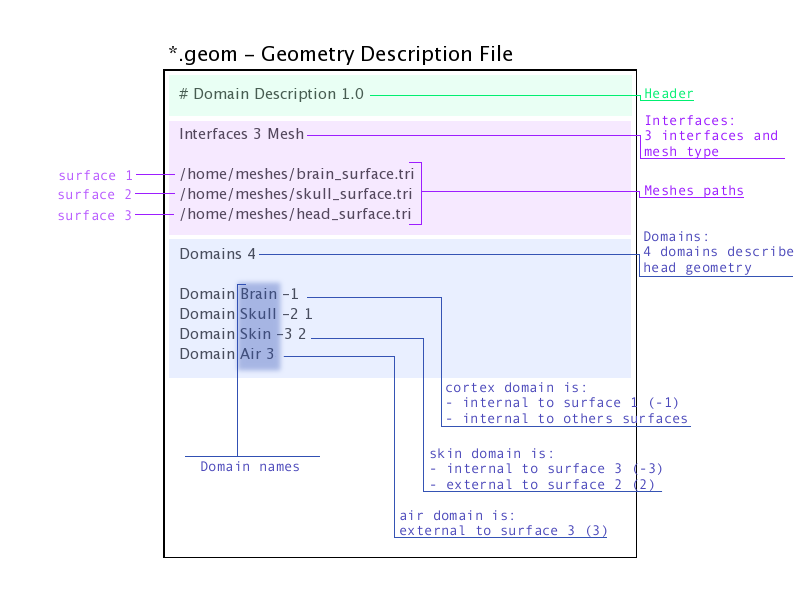
\includegraphics[height=9cm]{geom.png}}

\begin{note}
    Il est conseillé de noter la relation entre domaines et interfaces de la manière
    suivante (noter en premier la référence aux surfaces externes et en deuxième position la surface interne)~:

    \begin{tabular}{ll}
        Domain Brain -1              & \\
        Domain Skull \textbf{1 -2}	 &	\emph{et non pas Domain Skull -2 1} \\
        Domain Skin \textbf{2 -3}	 &	\emph{et non pas Domain Skin -3 2}  \\
        Domain Air 3                 &  \\
    \end{tabular}
\end{note}

\medskip

\begin{note}
    Les ``Meshes paths'' sont
    \begin{itemize}
        \item soit absolus (comme le montre le dessin)
        \item soit relatifs à l'endroit où on exécute les lignes de commandes
    \end{itemize}
    Seuls les formats suivants sont lus pour les surfaces maillées~:
    \begin{itemize}
        \item *.tri~: format TRI issu des premières versions de BrainVisa. Aussi lu par Anatomist.
        \item *.mesh~: format MESH issu des versions 3.0.2 et plus de BrainVisa. Aussi lu par Anatomist.
        \item *.vtk~: format de maillage VTK.
    \end{itemize}
\end{note}

%#############################################################
\section{Fichier de description des conductivités}
\label{sec:cond}

\noindent
Ce fichier décrit les valeurs des conductivités associées aux différents domaines déclarés dans le fichier de description de la
géométrie (section~\ref{sec:geom}).\\
Extension du fichier~: *.cond par convention.\\
\warning{bien respecter la casse entre les noms de domaines donnés dans le fichier de description de la géométrie et ceux
notés dans le fichier de description des conductivités !}

\centerline{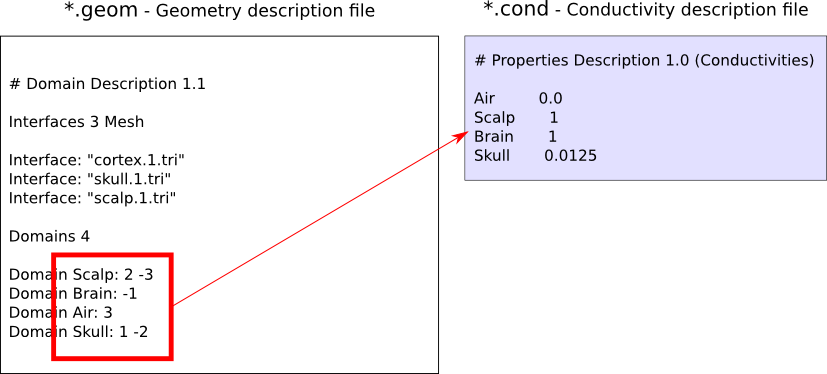
\includegraphics[height=9cm]{cond.png}}



%###################################################

\section{Descriptions des sources d'activité cérébrale}
Les sources sont définies par leur géométrie (position et orientation) et leur amplitude.
OpenMEEG peut traiter deux types de modèles de source: des dipôles isolés, ou bien des dipôles distribués.
Ces deux modèles sont décrits ci-dessous.

%-----------------------------------
\subsection{Position et orientation des sources}
\label{sec:dipoles}
%----
\subsubsection{Dipôles isolés}
\noindent
Les dipôles isolés sont représentés par un fichier texte, dans lequel à chaque ligne correspond un dipôle~:
\begin{itemize}
    \item les trois premiers nombres (séparés par un espace) sont les coordonnées cartésiennes de la position du dipôle,
    \item les trois derniers nombres (séparés par un espace) sont les coordonnées cartésiennes du vecteur normale donnant
           l'orientation du dipôle.
\end{itemize}
Extension de fichier~: *.dip ou *.txt.

\medskip

\noindent
Exemple d'un fichier décrivant 5 dipôles~:

\centerline{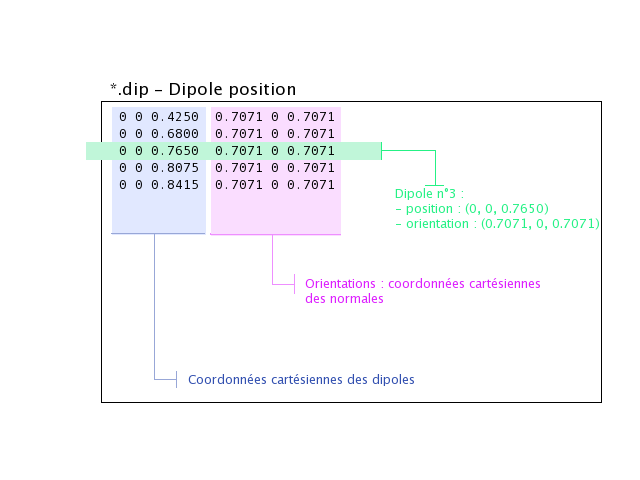
\includegraphics[height=9cm]{dipolePositions.png}}

\begin{note}
    les coordonnées sont définies dans le même repère que celui des maillages (repère de l'IRM en général)
\end{note}

%----
\subsubsection{Dipôles distribués}
Les dipôles distribués sont supportés sur une surface, de format *.tri, *.mesh ou *.vtk.
%-----------------------------------
\subsection{Activation des sources}
\label{sec:activ}

\noindent
Les fichiers d'activation des sources sont des fichiers texte. A une ligne correspond une source~:
\begin{itemize}
    \item dans le cas dipolaire, sont écrits sur la ième ligne les états d'activation du ième dipôle,
    \item dans le cas des sources distribuées, sont écrits sur la ième ligne les états d'activation du ième point du maillage
          des sources.
\end{itemize}

\medskip

\noindent
On trouve en colonne les temps auxquels sont associés les activations.

\medskip

\noindent
Exemple dans le cas dipolaire~:

\centerline{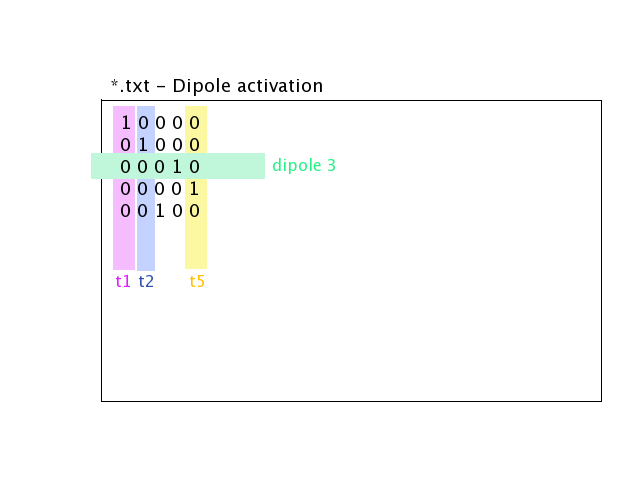
\includegraphics[height=9cm]{dipActiv.png}}

%###################################################

\section{Description des capteurs}
\label{sec:sensors}

\noindent
Les capteurs sont décrits par un fichier texte, dans laquelle chaque ligne contient la position du capteur,
et éventuellement d'autres informations telles que son label ou son orientation. Plus précisément, on dispose de 5 options pour définir les capteurs:
\begin{enumerate}
\item  1 ligne par capteur et 3 colonnes (typiquement pour les électrodes EEG ou des capteurs MEG sans orientation) :
	\begin{itemize}
		\item  les trois colonnes représentent les coordonnées cartésiennes du capteur
	\end{itemize}
\item  1 ligne par capteur et 4 colonnes (typiquement pour les électrodes EEG ou des capteurs MEG sans orientation) :
	\begin{itemize}
		\item   la première colonne contient le nom du capteur (label)
		\item les colonnes 2, 3 et 4  représentent les coordonnées cartésiennes du capteur
	\end{itemize}
\item 1 ligne par capteur et 6 colonnes (typiquement pour des capteurs MEG) :
	\begin{itemize}
		\item  les colonnes 1, 2  et 3  représentent les coordonnées cartésiennes du capteur
		\item  les colonnes 4, 5, et 6 représentent l'orientation du capteur
	\end{itemize}
\item  1 ligne par capteur et 7 colonnes (typiquement pour des capteurs MEG) :
	\begin{itemize}
		\item la première colonne contient le nom du capteur (label)
		\item les colonnes 2, 3  et 4  représentent les coordonnées cartésiennes du capteur
		\item les colonnes 5, 6, et 7 représentent l'orientation du capteur
	\end{itemize}
\item 1 ligne par point d'intégration pour chaque capteur, et 8 colonnes (typiquement pour des gradiomètres MEG ou des capteurs réalistes avec bobines) :
	\begin{itemize}
		\item  la première colonne contient le nom du capteur (label)
		\item les colonnes 2, 3  et 4  représentent les coordonnées cartésiennes du capteur
		\item  les colonnes 5, 6, et 7 représentent l'orientation du capteur
		\item  la colonne 8 contient le poids à appliquer pour l'intégration numérique (relative au nom du capteur)
	\end{itemize}

\end{enumerate}

Exemple de description de capteurs MEG:


% \centerline{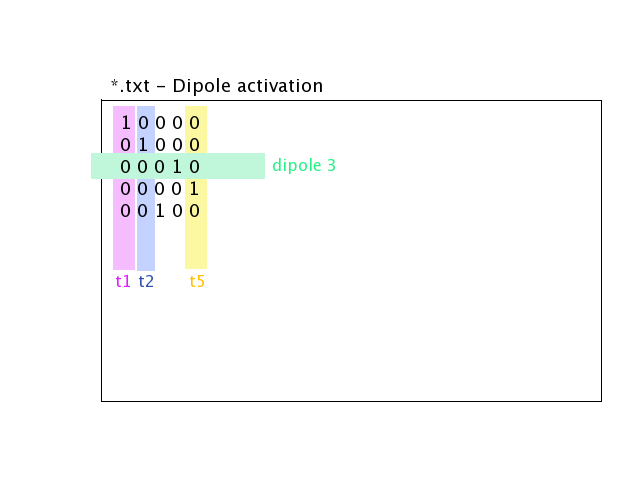
\includegraphics[height=9cm]{dipActiv.png}}
\centerline{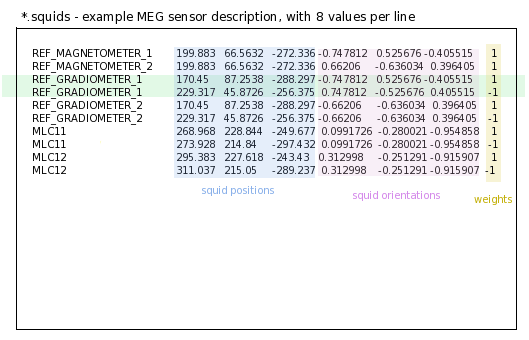
\includegraphics[height=9cm]{sensors-grad.png}}


\end{document}
